\begin{frame}{A Taxonomy of Repeated Games Models}
    \begin{figure}
        \tikzstyle{mybox} = [draw=gray!20, fill=white, very thick,
        rectangle, rounded corners, inner sep=10pt, inner ysep=10pt]
        \tikzstyle{fancytitle} = [fill=gray, text=white, rounded corners]
        \scalebox{0.7}{
        \begin{tikzpicture}
            \node [mybox] at (0, 0) (gen-mod){%
                \begin{minipage}{0.50\textwidth}
                    \vspace{-0.25cm}
                    \[ \Gamma^r = (N, \Theta, (D_i, S_i, u_i)_{i\in N}, q, p) \]
                \end{minipage}
            };
            \node [inner sep=0pt] (gen-mod-img) at (-4.4, 0.5){%
                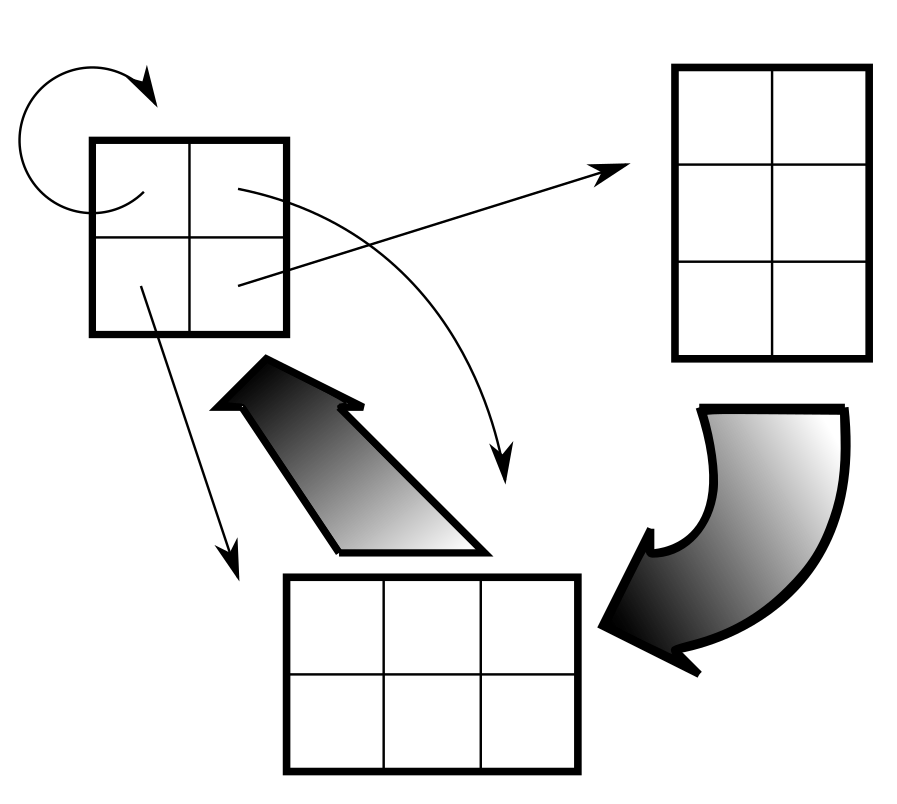
\includegraphics[width=0.25\textwidth]{img/stochastic.png}
            };
            
            \node [mybox] at (-4.5, -3) (mdp){%
                \begin{minipage}{0.40\textwidth}
                    {\color{green}Single-agent stochastic game}
                    \vspace{-0.25cm}
                    \[ |N| = 1. \]
                \end{minipage}
            };
            
            \node [mybox, draw=black] at (0, -7.5) (state){%
                \begin{minipage}{\textwidth}
                    {\color{green}At every round, every player knows the
                    current state of nature $\theta \in \Theta$.} \\
                    Informally, for each player $i \in N$, there exists some
                    state $w(s_i) \in \Theta$ such that the signal $s_i$ can
                    never occur unless the current state is $w(s_i)$.
                \end{minipage}
            };
            
            \node [mybox] at (4.5, -3.5) (std){%
                \begin{minipage}{0.60\textwidth}
                    \begin{itemize}
                        \item {\color{green}Only one possible state of
                        nature}
                        \[ |\Theta| = 1. \]
                        \item {\color{green}Players know all of each other's past
                        moves}
                        \[ S_i = \bigtimes_{j\in N-i} D_j. \]
                    \end{itemize}
                \end{minipage}
            };
            \node [inner sep=0pt] (gen-mod-img) at (7, -5.5){%
                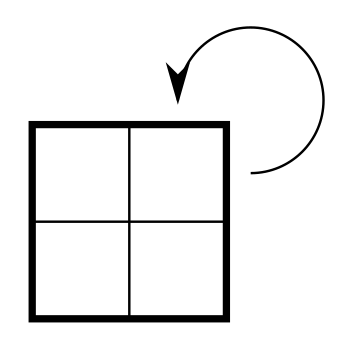
\includegraphics[width=0.20\textwidth]{img/std.png}
            };

            \node[fancytitle] at (gen-mod.north) {Stochastic Games (General Model)};
            \node[fancytitle] at (mdp.north) (mdp-title) {Markov Decision Processes};
            \node[fancytitle, fill=black] at (state.north) (state-title) {Complete State Information};
            \node[fancytitle] at (std.north) (std-title) {Standard Repeated Games};

            \draw[thick, -Latex] (gen-mod.west) -- (mdp-title.north);
            \draw[thick, -Latex] (gen-mod.south) -- (state-title.north);
            \draw[thick, -Latex] (gen-mod.east) -- (std-title.north);
        \end{tikzpicture}}
        \caption{A taxonomy of repeated game models.}
    \end{figure}
\end{frame}

\begin{frame}{Definition : Game with complete state information}

\metroset{block=fill}
\begin{block}{Definition}
A repeated game $\Gamma^r = (N,\Theta, (D_i,S_i,u_i)_{i\in N},q,p)$ has {\color{green}complete state information} if, at every round, every player knows the current state of nature. That is, there is a function $\omega_i:S_i \rightarrow \Theta$ know by each player such that:
\begin{equation*}
    \forall s \in S, \forall \theta, \hat{\theta} \in \Theta, \forall d \in D : p(s,\hat{\theta} | d,\theta) = 0 \text{ if } \hat{\theta} \neq \omega_i(s_i)
\end{equation*}
So the signal $s_i$ can never occur unless the current state is $\omega(s_i)$
\end{block}

\pause
\textbf{Example / Interpretation}

For the prisoner's dilema, if we assume that \alert{players make decision based only on the last move of their oponent}. We have four different state : $\Theta = \{([C,c]), ([C,d]), ([D,c]), ([D,d])\}$

\end{frame}

\begin{frame}{Definition : stationary}

\metroset{block=fill}
\begin{block}{definition}
In a repeated game, a game is said to be {\color{green}stationary} iff the move probabiliy depends only on the current state. That is there is a function $\tau_i : \Theta \rightarrow \Delta(D_i)$ such that:
\begin{equation*}
	\forall k, \forall s \in (S)^{\times k} : \sigma_i^{[k]}(\cdot | s) = \tau_i(\cdot | \omega_i(s_i^{[k]}))
\end{equation*}
\end{block}

\pause
\textbf{Example / Interpretation}

For the prisoner's dilema, a strategy is said to be stationary, if there is only one move possible for the player at each state $\theta$.

\note{
	Explain that this definition is only for game with complete state information
	
	Il faut connaître l'état pour etre stationnaire, si on ne connait pas l'état on ne pourra pas être stationnaire.
}
\end{frame}

\begin{frame}{Small example to understand complete state information}
\textit{Consider the prisoner's dilema game in a setting where player make decision based only on the last move of they adversary.} \note{This is contrary to decision theory to make this assumption. Some strategies can still be analysed in that setting. (tit-for-tat)}

\pause
$\Rightarrow$ 4 different states : $\Theta = \{([C,c]), ([C,d]), ([D,c]), ([D,d])\}$

\pause
If both player play the \textbf{tit-for-tat} strategy. {\color{green} We can represent } the game like that:

\begin{minipage}{0.7\linewidth}
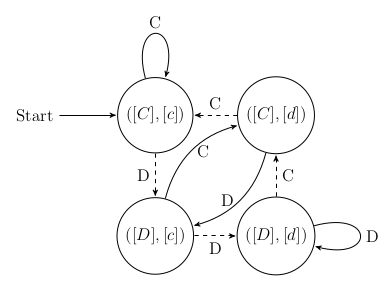
\includegraphics[width=0.9\linewidth]{img/titfortat.png}
\end{minipage}
\begin{minipage}{0.29\linewidth}
	\begin{itemize}
		\item Plain arrow if player 1 play tit-for-tat.
		\item Dashed arrow if player 1 play the opposite.
		\item Player 2 play tit-for-tat
	\end{itemize}
\end{minipage}
\end{frame}

\begin{frame}{Representation of the complate state information : Prisoner's Dilema}


\end{frame}


\begin{frame}{Analyze the game}
Let's $\nu_i$ be the \textit{expected $\delta$-discounted average} of player $i$ when beginning from the state $\theta \in \Theta$ when everyone plays according to $\tau$.
\begin{small}
\begin{align*}
\nu_i(\theta, \tau) &=   \sum_{d_i \in D_i} \tau_i(d_i|\theta) \cdot Y_i(\tau, d_i, \nu_i, \theta, \delta)\\
&= \sum_{d_i \in D_i} \tau_i(d_i|\theta) \sum_{d_{-i} \in D_{-i}} \tau_{-i}(d_{-i} |\theta) \left( (1-\delta) u_i(d_i,\theta) + \delta \sum_{\hat{\theta}} p(\hat{\theta}|d,\theta) \nu_i(\hat{\theta},\tau) \right)  \\
&= \text{max}_{d_i \in D_i} Y_i(\tau, d_i, \nu_i, \theta, \delta)
\end{align*}
\end{small}
\begin{small}
\begin{align*}
Y_i(\tau, d_i, \nu_i, \theta, \delta) = \sum_{d_{-i} \in D_{-i}} \tau_{-i}(d_{-i} |\theta) \left( (1-\delta) u_i(d_i,\theta) + \delta \sum_{\hat{\theta}} p(\hat{\theta}|d,\theta) \nu_i(\hat{\theta},\tau) \right)
\end{align*}
\end{small}
This expression can be interpreted as the gain of player $i$ if he played the move $d_i$ once if at state $\theta$ everyone else follows $\tau$.
\end{frame}

\begin{frame}{Let's go back to the prisonner's dilema for a small example}
For a given $0 \leq \delta < 1$ we have the followin $\delta$-discounted payoff for player 1
	\begin{align*}
		\nu_1([C],[c]) &= (1-\delta) \cdot 1 + \delta \cdot \nu_1([C],[c])\\
		\nu_1([D],[c]) &= (1-\delta) \cdot -1 + \delta \cdot \nu_1([C],[c])\\
		\nu_1([C],[d]) &= (1-\delta) \cdot 2 + \delta \cdot \nu_1([C],[c])\\
		\nu_1([D],[d]) &= (1-\delta) \cdot 0 + \delta \cdot \nu_1([C],[c])
	\end{align*}
\pause
The solution are imediate:
\begin{align*}
	\nu_1([C],[c]) &= 1\\
	\nu_1([D],[c]) &= \frac{2\delta - 1}{1+\delta}\\
	\nu_1([C],[d]) &= \frac{2-\delta}{1+\delta}\\
	\nu_1([D],[d]) &= 0
\end{align*}
\end{frame}

\begin{frame}
	Then, to ensure that $\tau$ is an equilibrium of the repeated game, we must verify the equation $\nu_i(\theta) = \text{max}_{d_i \in D_i} Y_i(\tau, d_i, \nu_i, \theta, \delta)$. That is to ensure that the follwing inequalities are satisfied.
\begin{align*}
	\nu_1([C],[c]) &\geq (1-\delta)2 + \delta \nu_1([D],[c]) = \nu_1([C],[d]) \quad \text{Doing D instead of C}\\
	\nu_1([D],[c]) &\geq (1-\delta)0 + \delta \nu_1([D],[d]) = 0 \qquad \text{Doing D instead of C}\\
	\nu_1([C],[d]) &\geq (1-\delta)1 + \delta \nu_1([C],[c]) = 1 \qquad \text{Doing C instead of D}\\
	\nu_1([D],[d]) &\geq (1-\delta)(-1) + \delta \nu_1([C],[d]) = \nu_1([D],[c]) \quad \text{Doing C instead of D}
\end{align*}

\pause
\begin{itemize}
	\item For $\delta = 0.5$ : equilibrium reached
	\item For $\delta \leq 0.5$ : We play as for the non repetitive Prisoner's dilemma (search for immediate reward).
	\item For $\delta \geq 0.5$ : If we know that the other is going to play Tit-for-Tat, we should always play cooperate.
\end{itemize}

\end{frame}
